% !TEX root =  main.tex
By Section \ref{Numerical methods for computing the Casimir energy}, to compute the Casimir energy, it is necessary to evaluate the term
$\log\det(\mathsf{V}(\mathrm{i}k)\tilde{\mathsf{V}}(\mathrm{i}k)^{-1})$ 
with different values of $k$. In this section, several efficient methods will be introduced to compute this log determinant.

The log determinant of the matrix $\mathsf{V}(\mathrm{i}k)\tilde{\mathsf{V}}(\mathrm{i}k)^{-1}$ is equal to the sum of the logarithm of the eigenvalues of 
$\mathsf{V}(\mathrm{i}k)\tilde{\mathsf{V}}(\mathrm{i}k)^{-1}$. Since $\tilde{\mathsf{V}}(\mathrm{i}k)$ is a compact perturbation of $\mathsf{V}(\mathrm{i}k)$,
most of the eigenvalues of the matrix $\mathsf{V}(\mathrm{i}k)\tilde{\mathsf{V}}(\mathrm{i}k)^{-1}$ are close to 1 
(shown in Figure \ref{eigenvalues of VVtilde}) and contribute little to the value of the Casimir energy. Hence, we do not need to compute all eigenvalues but only
the extremal ones, making subspace methods such as Krylov solvers attractive for this problem.

In what follows we demonstrate and compare iterative solver approaches based on the inverse free Krylov subspace method \cite{golub2002inverse} \cite{money2005algorithm}, 
and based on standard Arnoldi iterations \cite{arnoldi1951principle}.
We will also discuss on acceleration strategy which is based on the idea of recycling projection bases from one quadrature point to the next. 


\begin{figure}[H]
    \centering
    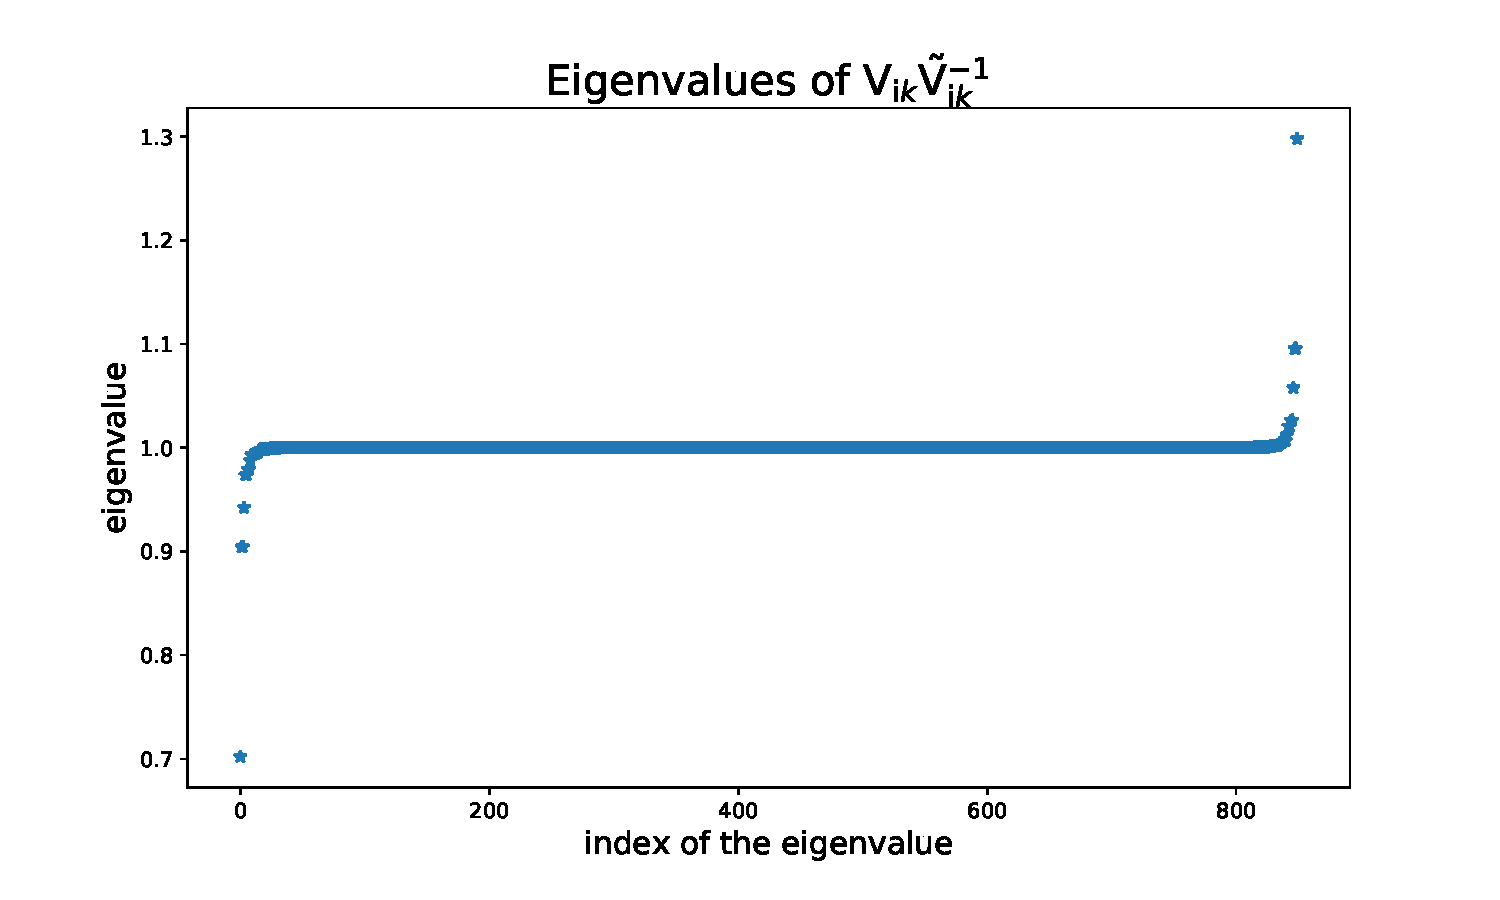
\includegraphics[scale = 0.4]{figures/eigenvalue_of_VVtilde.pdf}
    \caption{The eigenvalues of the matrix $\mathsf{V}(\mathrm{i}k)\tilde{\mathsf{V}}(\mathrm{i}k)^{-1}$ when $\mathrm{i}k = 0.8\mathrm{i}$.
    The scatterers are two spheres with equal radii $r_{1} = r_{2} = 1$ and the minimal distance between them is $Z = 0.5$. The grid size of the mesh is $h = 0.1$.}
    \label{eigenvalues of VVtilde}
\end{figure}

\subsection{Method I: Inverse-free Krylov subspace method}

Consider the eigenvalue problem: 
\begin{align} \label{EP}
    \mathsf{V}(\mathrm{i}k)\tilde{\mathsf{V}}(\mathrm{i}k)^{-1}\boldsymbol{x} = \lambda\boldsymbol{x},
\end{align}
where $\lambda$ is the eigenvalue and $\boldsymbol{x}$ is the corresponding eigenvalue. This eigenvalue problem is equivalent to the following generalized eigenvalue problem:
\begin{align}\label{GEP}
    \mathsf{V}(\mathrm{i}k)\tilde{\boldsymbol{x}}) = \lambda \tilde{\mathsf{V}}(\mathrm{i}k)\tilde{\boldsymbol{x}}.
\end{align}


An important property of this problem is that as we are only interested in $ik$ along the imaginary axis, the corresponding matrix $\tilde{\mathrm{V}}(\mathrm{i}k)$ is positive definite in the scalar case,
and $\mathrm{V}(\mathrm{i}k)$ is still symmetric.

In \cite{golub2002inverse}\cite{money2005algorithm},
the authors proposed an inverse-free Krylov subspace method for computing a few extreme eigenvalues of the symmetric definite generalized eigenvalue problem.
The following algorithms summarizes the method.

\begin{algorithm}[H]
    \SetAlgoLined
    Input: Symmetric matrix $A\in\mathbb{R}^{n\times n}$, s.p.d matrix $B\in\mathbb{R}^{n\times n}$, an initial approximation $\boldsymbol{x}$ with $||\boldsymbol{x}|| = 1$,
    a given shift $\rho$ and the dimension of the Krylov subspace $m\geq 1$\\
    Output: A set of approximate eigenvalues of $A\boldsymbol{x} = \lambda B\boldsymbol{x}$ and associated eigenvectors.\\
    \begin{algorithmic}[1]
        
        \STATE Construct a basis $Z_{m}$ for the Krylov subspace $K_{m} = \text{span}(\boldsymbol{x}, (A - \rho B)\boldsymbol{x}, \dots, (A - \rho B)^{m-1}\boldsymbol{x})$ with dimension $m$
        \STATE Project $A$ and $B$ on $Z$: $A_{m} = Z_{m}^{T}(A - \rho B)Z_{m}$, $B_{m} = Z_{m}^{T}BZ_{m}$
        \STATE Compute all the eigenpairs $\{(\tilde{\lambda}_{i}, \boldsymbol{x}_{i})\}_{i = 1, \dots, m}$ for the matrix pencil $(A_{m}, B_{m})$
        \STATE Reverse the shift to obtain $\lambda_{i} = \tilde{\lambda}_{i} + \rho$.
        \end{algorithmic}
    \caption{Inverse-free Krylov subspace method for computing multiple extreme eigenvalues of the generalized eigenvalue problem $A\boldsymbol{x} = \lambda B\boldsymbol{x}$}
    \label{Alg for computing the evals kry}
    \end{algorithm}
   
    
{\color{red} Why do you say extreme? Isn't the algorithm finding eigenvalues close to the shift?} {\color{teal} Algorithm \ref{Alg for computing the evals kry} approximates $m$ eigenvalues close to the shift $\rho$ 
for the matrix pencil $(A,B)$}, where $m$ is the dimension of the 
Krylov subspace $K_{m}$ in Step 1, Algorithm \ref{Alg for computing the evals kry}. The question is what shift strategy to use for $\rho$. In numerical experiments it turned
out that for the KSSF problem choosing $\rho=1$ sufficiently approximate the eigenvalues that have the main contribution to $\log\det(\mathsf{V}(\mathrm{i}k_{j})\tilde{\mathsf{V}}(\mathrm{i}k_{j})^{-1}) $.

The main cost of the inverse free Krylov subspace method is the computation of the Krylov subspace and the projection of the matrices $A$ and $B$. In our case these are large dense matrices representing
integral operators. In order to reduce the cost of computing a Krylov subspace basis for each wavenumber $\mathrm{i}k$ we can use a recycling strategy based on the idea that a Krylov subspace for a previous quadrature
point in the KSSF integral will be a good approximation to a Krylov subspace for the current quadrature point. We initially compute a Krylov basis for the wavenumber $\mathrm{i}k_{1}$ associated with the first
quadrature point. We then extract several eigenvectors associated with the extremal eigenvalues based on Algorithm \ref{Alg for computing the evals kry} and then orthogonalize to obtain an initial approximation
basis for the wavenumber $ik_2$. For this wavenumber we project the matrices onto the recycled basis, compute approximate eigenpairs $(\tilde{\lambda}_i, \tilde{\mathbf{x}}_i)$ and then extend the subspace
basis with the residuals $\boldsymbol{r}_i = \mathrm{V}(\mathrm{i}k)\tilde{\boldsymbol{x}}_i - \tilde{\lambda}_i\tilde{\mathrm{V}}(\mathrm{i}k)\tilde{\boldsymbol{x}}_i$. With the extended subspace we recompute the eigenpairs for the second wavenumber's
case and extract eigenvectors as starting basis for the third wavenumber, and so on.


%For the second wavenumber, we initially compute the approximated eigenvalues ($\{\tilde{\lambda}_{i}\}$) and eigenvectors $\left(\{\tilde{\boldsymbol{x}}_{i}\}\right)$ with the 
%recycled subspace and use the residual vectors $\left(\{\boldsymbol{r}_{i}\},\ \text{where}\ \boldsymbol{r}_{i} = \mathsf{V}_{\mathrm{i}k_{2}}\tilde{\boldsymbol{x}}_{2} - \tilde{\lambda}_{i}\tilde{\mathsf{V}}_{\mathrm{i}k_{1}}\tilde{\boldsymbol{x}}_{i}\right)$
%to expand the temporary basis. With the expanded subspace, we recompute the eigenpairs for the second wavenumber's case and extract the resulting eigenvectors for the 
%third wavenumber and so on. This modified inverse-free Krylov subspace method based on the recycled subspace is completely described in 
%Algorithm \ref{Alg for computing the evals kry recycled}.
%
%\begin{algorithm}[H]
%    \SetAlgoLined
%    Input: $N$: the number of matrix pencils ($A^{(i)}, B^{(i)}$), an initial approximation $\boldsymbol{x}$ with $||\boldsymbol{x}|| = 1$, the shift $\rho = 1$, the dimension of Krylov subspace $m\geq 1$ and the number of chosen extreme eigenvalues $\{s_{i}\}_{i}$, for $i = 1, 2, \dots, (N-1)$\\
%    Output: The approximated extreme eigenvalues of $A\boldsymbol{x} = \lambda B\boldsymbol{x}$\\
%
%    \begin{algorithmic}[1]
%        \STATE When $i = 1$:
%        \begin{itemize}
%            \item[(a)] Compute the basis $Z_{m}^{(1)}$ for the Krylov subspace $K_{m}^{(1)} = \text{span}\left(\boldsymbol{x}, (A^{(1)} - \rho B^{(1)})\boldsymbol{x}, \dots, (A^{(1)} - \rho B^{(1)})^{m-1}\boldsymbol{x}\right)$ with dimension $m$
%            
%            \item[(b)] Project $A^{(1)}$ and $B^{(1)}$ on $Z_{m}^{(1)}$: 
%            $A_{m}^{(1)} = Z_{m}^{(1)H}(A^{(1)} - \rho B^{(1)})Z_{m}^{(1)},\  B_{m}^{(1)} = Z_{m}^{(1)H}B^{(1)}Z_{m}^{(1)}$
%
%    
%            \item[(c)] Compute the eigenvalues $\boldsymbol{\lambda}^{(1)} = \{\lambda_{1}^{(1)}, \dots, \lambda_{m}^{(1)}\}$ and eigenvectors $\boldsymbol{X}_{m}^{(1)} = \left[\boldsymbol{x}_{1}^{(1)}, \dots, \boldsymbol{x}_{m}^{(1)}\right]$ for $A_{m}^{(1)}\boldsymbol{x} = \lambda B_{m}^{(1)}\boldsymbol{x}$ and note that the approximated eigenvalues for $A^{(1)}\boldsymbol{x} = \lambda B^{(1)}\boldsymbol{x}$ are $\{\lambda_{1}^{(1)}+\rho, \dots, \lambda_{m}^{(1)}+\rho\}$
%            
%            \item[(d)] Extract $s_{1}$ eigenvectors from $\boldsymbol{X}_{m}^{(1)}$, which correspond to $s_{1}$ extreme eigenvalues and relabel them as $\boldsymbol{X}_{s_{1}}^{(1)} = \left[\boldsymbol{x}_{1}^{(1)}, \dots, \boldsymbol{x}_{s_{1}}^{(1)}\right]$
%            
%            \item[(e)] Recover the eigenvectors for$A^{(1)}\boldsymbol{x} = \lambda B^{(1)}\boldsymbol{x}$ by computing $Z_{m}^{(1)}\boldsymbol{X}_{s_{1}}^{(1)}$ and orthogonalize it to obtain the temporary basis $\tilde{Z}_{s_{1}}^{(2)} = \text{orth}\left(Z_{m}^{(1)}\boldsymbol{X}_{s_{1}}^{(1)}\right)$ for the second matrix pencil ($A^{(2)}, B^{(2)}$)
%        \end{itemize}
%        
%        \STATE When $i = 2$:
%        \begin{itemize}
%            \item[(a)] Project $A^{(2)}$ and $B^{(2)}$ on $\tilde{Z}_{s_{1}}^{(2)}$: 
%            $\tilde{A}_{s_{1}}^{(2)} = \tilde{Z}_{s_{1}}^{(2)H}A^{(2)} \tilde{Z}_{s_{1}}^{(2)},  \tilde{B}_{s_{1}}^{(2)} = \tilde{Z}_{s_{1}}^{(2)H}B^{(2)}\tilde{Z}_{s_{1}}^{(2)}$
%
%            \item[(b)] Compute the eigenvalues $\tilde{\boldsymbol{\lambda}}^{(2)} = \{\tilde{\lambda}_{1}^{(2)}, \dots, \tilde{\lambda}_{s_{1}}^{(2)}\}$ and eigenvectors $\tilde{\boldsymbol{X}}_{s_{1}}^{(2)} = \left[\tilde{\boldsymbol{x}}_{1}^{(2)}, \dots, \tilde{\boldsymbol{x}}_{s_{1}}^{(2)}\right]$ for $\tilde{A}_{s_{1}}^{(2)}\boldsymbol{x} = \lambda \tilde{B}_{s_{1}}^{(1)}\boldsymbol{x}$
%            
%            \item[(c)] Compute the residuals $\boldsymbol{r}_{i}^{(2)} = A^{(2)}\tilde{Z}_{s_{1}}^{(2)}\tilde{\boldsymbol{x}}_{i}^{(2)} - \tilde{\lambda}_{i}^{(2)}B^{(2)}\tilde{Z}_{s_{1}}^{(2)}\tilde{\boldsymbol{x}}_{i}^{(2)}$ for $i = 1, 2, \dots, s_{1}$ and denote $\boldsymbol{r}^{(2)} = \left[\boldsymbol{r}_{1}^{(2)}, \dots, \boldsymbol{r}_{s_{1}}^{(2)}\right]$
%            
%            \item[(d)] Construct the basis $Z_{2s_{1}}^{(2)}$ for $(A^{(2)}, B^{(2)})$ by extending the temporary basis $\tilde{Z}_{s_{1}}^{(2)}$ with the residues $\boldsymbol{r}^{(2)}$ and orthogonalizing the extended subspace: $Z_{2s_{1}}^{(2)} = \left[\tilde{Z}_{s_{1}}^{(2)}, \tilde{\boldsymbol{r}}^{(2)}\right]$, where $\tilde{\boldsymbol{r}}^{(2)} = \text{orth}\left(\boldsymbol{r}^{(2)}\right)$
%            
%            \item[(e)] Project $A^{(2)}$ and $B^{(2)}$ on $Z_{2s_{1}}^{(2)}$: 
%            \begin{align*}
%                A_{2s_{1}}^{(2)} &= Z_{2s_{1}}^{(2)H}A^{(2)} Z_{2s_{1}}^{(2)} = \begin{bmatrix}
%                 \tilde{A}_{s_{1}}^{(2)} & \tilde{Z}_{s_{1}}^{(2)H}A^{(2)} \tilde{\boldsymbol{r}}^{(2)}\\
%                 \tilde{\boldsymbol{r}}^{(2)H} A^{(2)} \tilde{Z}_{s_{1}}^{(2)} & \tilde{\boldsymbol{r}}^{(2)H} A^{(2)} \tilde{\boldsymbol{r}}^{(2)}
%                \end{bmatrix}, \\
%                B_{2s_{1}}^{(2)} &= Z_{2s_{1}}^{(2)H}B^{(2)}Z_{2s_{1}}^{(2)} = \begin{bmatrix}
%                 \tilde{B}_{s_{1}}^{(2)} & \tilde{Z}_{s_{1}}^{(2)H}B^{(2)} \tilde{\boldsymbol{r}}^{(2)}\\
%                 \tilde{\boldsymbol{r}}^{(2)H} B^{(2)} \tilde{Z}_{s_{1}}^{(2)} & \tilde{\boldsymbol{r}}^{(2)H} B^{(2)} \tilde{\boldsymbol{r}}^{(2)}
%                \end{bmatrix}
%            \end{align*}
%            \item[(f)] Repeat Step 1(c)-(e) for these projected matrices to compute the approximated eigenvalues $\boldsymbol{\lambda}^{(2)} = \{\lambda_{1}^{(2)}, \dots, \lambda_{2s_{1}}^{(2)}\}$  and eigenvectors $\boldsymbol{X}_{2s_{1}}^{(2)} = \left[\boldsymbol{x}_{1}^{(2)}, \dots, \boldsymbol{x}_{2s_{1}}^{(2)}\right]$ for $\left( A_{2s_{1}}^{(2)},  B_{2s_{1}}^{(2)}\right)$ and obtain the temporary basis $\tilde{Z}_{s_{2}}^{(3)}$ for the third matrix pencil $\left(A^{(3)}, B^{(3)}\right)$
%        \end{itemize}
%        
%        \STATE For $i = 3, \dots, N$, repeat the Step 2 to compute the approximated eigenvalues $\boldsymbol{\lambda}^{(i)} = \{\lambda_{1}^{(i)}, \dots, \lambda_{2s_{i-1}}^{(i)}\}$  and eigenvectors $\boldsymbol{X}_{2s_{i-1}}^{(i)} = \left[\boldsymbol{x}_{1}^{(i)}, \dots, \boldsymbol{x}_{2s_{i-1}}^{(i)}\right]$ for each matrix pencil
%        \end{algorithmic}
%    \caption{Inverse-free recycled Krylov subspace method for sequences of generalized eigenvalue problems $A^{(i)}\boldsymbol{x} = \lambda B^{(i)}\boldsymbol{x}$}
%    \label{Alg for computing the evals kry recycled}
%    \end{algorithm}    

%In this case, the value of 
%$\log\det(\mathsf{V}_{\mathrm{i}k_{j}}\tilde{\mathsf{V}}_{\mathrm{i}k_{j}}^{-1})$ can be approximated by 
%\begin{equation}
%    \log\det(\mathsf{V}_{\mathrm{i}k_{j}}\tilde{\mathsf{V}}_{\mathrm{i}k_{j}}^{-1})  \approx
%      \begin{cases}
%        \sum_{i = 1}^{m} \log\left(\lambda_{i}^{(j)}\right) & j = 1\\
%        \sum_{i = 1}^{2s_{j-1}} \log\left(\lambda_{i}^{(j)}\right) & j = 2, \dots, N
%      \end{cases}       
%  \end{equation}

\subsection{Method II: Standard Arnoldi method}

An alternative to the inverse-free projection method is to use standard Arnoldi to construct the Krylov subspace  
$K_{m}(\mathsf{V}(\mathrm{i}k)\tilde{\mathsf{V}}(\mathrm{i}k)^{-1}, \boldsymbol{b})$, where $\boldsymbol{b}$ is some 
initial vector and $m$ is the dimension of this Krylov subspace, and to then compute the eigenvalues of the resulting projected Hessenberg matrix $H_m$ (see \cite{saad2011numerical}).

The computation of $\tilde{\mathsf{V}}(\mathrm{i}k)^{-1}\boldsymbol{y}$ for some vector $y$ can be efficiently implemented since $\tilde{\mathsf{V}}(\mathrm{i}k)$ is simply a block-diagonal matrix with the
discretised single-layer potentials for each domain as block matrices. Hence, we just need to compute LU decompositions of these operators, and not of the whole system matrix.
Similarly to the inverse free method we can again use a recycling approach based on the same idea of expanding our subspace with computed residuals, but now projecting
$\mathsf{V}(\mathrm{i}k)\tilde{\mathsf{V}}(\mathrm{i}k)^{-1}$ onto the recycled space.


%
%Afterwards, we implement the standard Arnoldi iteration to obtain the orthogonal basis of 
%this order-$m$ Krylov subspace and project the matrix $\mathsf{V}_{\mathrm{i}k}\tilde{\mathsf{V}}_{\mathrm{i}k}^{-1}$ onto this basis. 
%This projection matrix is called the Hessenberg matrix and we denote it as $H_{m}$. By \cite{saad2011numerical}, the eigenvalues of $H_{m}$ (which are also 
%called Ritz eigenvalues) can give good approximations on extreme eigenvalues of $\mathsf{V}_{\mathrm{i}k}\tilde{\mathsf{V}}_{\mathrm{i}k}^{-1}$.
%The following algorithm lists the general steps described above.


%\begin{algorithm}[H]
%    \SetAlgoLined
%    Input: Block matrix $A\in\mathbb{R}^{n\times n}$, diagonal block matrix $B\in\mathbb{R}^{n\times n}$ and the dimension of the Krylov subspace $m\geq 1$\\
%    Output: The approximated extreme eigenvalue of $AB^{-1}\boldsymbol{x} = \mu \boldsymbol{x}$\\
%    \begin{algorithmic}[1]
%        \STATE Use standard Arnoldi method to compute the Hessenberg matrix $H_{m}$ of $AB^{-1}$
%        \STATE Compute all the eigenpairs $\{(\mu_{i}, \boldsymbol{x}_{i})\}_{i = 1, \dots, m}$ of $H_{m}$
%        \end{algorithmic}
%    \caption{Standard Arnoldi method for computing multiple extreme eigenvalues of the eigenvalue problem $AB^{-1}\boldsymbol{x} = \mu\boldsymbol{x}$}
%    \label{Alg for arno method}
%    \end{algorithm}
%
%\begin{remark}
%    During the Arnoldi iteration process, one needs to multiply the inverse matrix $\tilde{\mathsf{V}}_{\mathrm{i}k}^{-1}$ with some vector 
%$\boldsymbol{v} = \begin{bmatrix}\boldsymbol{v}_{1}\\ \vdots \\ \boldsymbol{v}_{N} \end{bmatrix}$. In order to avoid directly computing 
%the matrix inversion, one can firstly compute LU decomposition for each diagonal 
%block matrix $\mathsf{V}_{ii}(\mathrm{i}k) = \mathsf{L}_{ii}\mathsf{U}_{ii} $, for $i = 1, 2, \dots, N$, where $\mathsf{L}_{ii}$ and $\mathsf{U}_{ii}$ are lower and upper triangular matrices, 
%respectively and solve the linear system $\mathsf{L}_{ii}\mathsf{U}_{ii}\boldsymbol{x}_{i} = \boldsymbol{v}_{i}$ for $i = 1, 2, \dots, N$. Finally, the resulting 
%vector is $\boldsymbol{x} = \begin{bmatrix}\boldsymbol{x}_{1}\\ \vdots \\ \boldsymbol{x}_{1} \end{bmatrix}$.
%\end{remark}


%By denoting the the eigenvalues of $H_{m}$ as $\{\mu_{i}\}_{i = 1, \dots, m}$, the value of  
%$\log\det(\mathsf{V}_{\mathrm{i}k}\tilde{\mathsf{V}}_{\mathrm{i}k}^{-1})$ can be approximated by
%\begin{align*}
%    \log\det(\mathsf{V}_{\mathrm{i}k}\tilde{\mathsf{V}}_{\mathrm{i}k}^{-1}) \approx \sum_{i = 1}^{m}\log\left(\mu_{i}\right).
%\end{align*}
%
%Same with the inverse-free Krylov subspace method, one can also recycle the eigenvectors associated with the extreme eigenvalues from the initial subspace 
%for the first wavenumber, expand it with some vectos (In Algorithm \ref{Alg for computing the evals kry recycled}, they are residual vectors) and 
%use the complemented basis for the second wavenumber's case. Algorithm \ref{Alg for computing the evals arno recycled} summarizes the whole steps for this 
%recycling process. 
%
%\begin{algorithm}[H]
%    \SetAlgoLined
%    Input: $N$: the number of matrices $A^{(i)}\left(B^{(i)}\right)^{-1}$, where $A^{(i)}$ are block matrices and $B^{(i)}$ are diagonal block matrices, an initial approximation $\boldsymbol{x}$ with $||\boldsymbol{x}|| = 1$, the shift $\rho = 1$, the dimension of Krylov subspace $m\geq 1$ and the number of chosen extreme eigenvalues $\{s_{i}\}_{i}$, for $i = 1, 2, \dots, (N-1)$\\
%    \vspace{0.5cm}
%    \begin{algorithmic}[1]
%        \STATE When $i = 1$:
%        \begin{itemize}
%            
%            \item[(a)]Apply the standard Arnoldi method to compute the Arnoldi vectors $Z_{m}^{(1)}$ and Hessenberg matrix $H_{m}^{(1)}$ for $A^{(1)}\left(B^{(1)}\right)^{-1}$, which satisfies $H_{m}^{(1)} = Z_{m}^{(1)H}\left(A^{(1)}\left(B^{(1)}\right)^{-1}\right)Z_{m}^{(1)}$
%    
%            \item[(b)] Compute the eigenvalues $\boldsymbol{\mu}^{(1)} = \{\mu_{1}^{(1)}, \dots, \mu_{m}^{(1)}\}$ and eigenvectors $\boldsymbol{X}_{m}^{(1)} = \left[\boldsymbol{x}_{1}^{(1)}, \dots, \boldsymbol{r}_{m}^{(1)}\right]$ for $H_{m}^{(1)}$
%            
%            \item[(c)] Extract $s_{1}$ eigenvectors from $\boldsymbol{X}_{m}^{(1)}$, which correspond to $s_{1}$ extreme eigenvalues and relabel them as $\boldsymbol{X}_{s_{1}}^{(1)} = \left[\boldsymbol{x}_{1}^{(1)}, \dots, \boldsymbol{x}_{s_{1}}^{(1)}\right]$
%            
%            \item[(d)] Recover the eigenvectors for $A^{(1)}\left(B^{(1)}\right)^{-1}x = \mu x$ by computing $Z_{m}^{(1)}\boldsymbol{X}_{s_{1}}^{(1)}$ and orthogonalize it to obtain the temporary basis $\tilde{Z}_{s_{1}}^{(2)} = \text{orth}\left(Z_{m}^{(1)}\boldsymbol{X}_{s_{1}}^{(1)}\right)$ for the second eigenvalue problem $A^{(2)}\left(B^{(2)}\right)^{-1}\boldsymbol{x} = \lambda \boldsymbol{x}$
%        \end{itemize}
%        
%        \STATE When $i = 2$:
%        \begin{itemize}
%            \item[(a)] Project $A^{(2)}\left(B^{(2)}\right)^{-1}$ on $\tilde{Z}_{s_{1}}^{(2)}$: 
%            \begin{align*}
%                \tilde{H}_{s_{1}}^{(2)} &= \tilde{Z}_{s_{1}}^{(2)H}\left(A^{(2)}\left(B^{(2)}\right)^{-1}\right) \tilde{Z}_{s_{1}}^{(2)}
%            \end{align*}
%            
%            \item[(b)] Compute the eigenvalues $\tilde{\boldsymbol{\mu}}^{(2)} = \{\tilde{\mu}_{1}^{(2)}, \dots, \tilde{\mu}_{s_{1}}^{(2)}\}$ and eigenvectors $\tilde{\boldsymbol{X}}_{s_{1}}^{(2)} = \left[\tilde{\boldsymbol{x}}_{1}^{(2)}, \dots, \tilde{\boldsymbol{x}}_{s_{1}}^{(2)}\right]$ for $A^{(2)}\left(B^{(2)}\right)^{-1}x = \lambda x$
%            
%            
%            \item[(c)] Compute the residuals $\boldsymbol{r}_{i}^{(2)} = \left(A^{(2)}\left(B^{(2)}\right)^{-1}\right)\tilde{Z}_{s_{1}}^{(2)}\tilde{\boldsymbol{x}}_{i}^{(2)} - \tilde{\mu}_{i}^{(2)}\tilde{Z}_{s_{1}}^{(2)}\tilde{\boldsymbol{x}}_{i}^{(2)}$, for $i = 1, 2, \dots, s_{1}$ and denote $\boldsymbol{r}^{(2)} = \left[\boldsymbol{r}_{1}^{(2)}, \dots, \boldsymbol{r}_{s_{1}}^{(2)}\right]$
%            
%            \item[(d)] Construct the basis $Z_{2s_{1}}^{(2)}$ for $A^{(2)}\left(B^{(2)}\right)^{-1}$ by extending the temporary basis $\tilde{Z}_{s_{1}}^{(2)}$ with the residues $\boldsymbol{r}^{(2)}$ and orthogonalizing the extended subspace: $Z_{2s_{1}}^{(2)} = \left[\tilde{Z}_{s_{1}}^{(2)}, \tilde{\boldsymbol{r}}^{(2)}\right]$, where $\tilde{\boldsymbol{r}}^{(2)} = \text{orth}\left(\boldsymbol{r}^{(2)}\right)$
%            
%            \item[(e)] Project $A^{(2)}\left(B^{(2)}\right)^{-1}$ on $Z_{2s_{1}}^{(2)}$: 
%            \begin{align*}
%                H_{2s_{1}}^{(2)} = Z_{2s_{1}}^{(2)H}\left(A^{(2)}\left(B^{(2)}\right)^{-1}\right) Z_{2s_{1}}^{(2)} = \begin{bmatrix}
%                 \tilde{H}_{s_{1}}^{(2)} & \tilde{Z}_{s_{1}}^{(2)H}\left(A^{(2)}\left(B^{(2)}\right)^{-1}\right) \tilde{\boldsymbol{r}}^{(2)}\\
%                 \tilde{\boldsymbol{r}}^{(2)H}\left(A^{(2)}\left(B^{(2)}\right)^{-1}\right) \tilde{Z}_{s_{1}}^{(2)} & \tilde{\boldsymbol{r}}^{(2)H}\left(A^{(2)}\left(B^{(2)}\right)^{-1}\right) \tilde{\boldsymbol{r}}^{(2)}
%                \end{bmatrix}
%            \end{align*}
%            \item[(f)] Repeat Step 1(c)-(e) for the projected matrix $ H_{2s_{1}}^{(2)}$ to compute the approximated eigenvalues $\boldsymbol{\mu}^{(2)} = \{\mu{1}^{(2)}, \dots, \mu{2s_{1}}^{(2)}\}$  and eigenvectors $\boldsymbol{X}_{2s_{1}}^{(2)} = \left[\boldsymbol{x}_{1}^{(2)}, \dots, \boldsymbol{x}_{2s_{1}}^{(2)}\right]$ and obtain the temporary basis $\tilde{Z}_{s_{2}}^{(3)}$ for the third eigenvalue problem $A^{(3)}\left(B^{(3)}\right)^{-1}x = \lambda x$
%        \end{itemize}
%        
%        \STATE For $i = 3, \dots, N$, repeat the Step 2 to compute the approximated eigenvalues $\boldsymbol{\mu}^{(i)} = \{\mu_{1}^{(i)}, \dots, \mu_{2s_{i-1}}^{(i)}\}$  and eigenvectors $\boldsymbol{X}_{2s_{i-1}}^{(1)} = \left[\boldsymbol{x}_{1}^{(i)}, \dots, \boldsymbol{x}_{2s_{i-1}}^{(i)}\right]$ for each eigenvalue problem
%        \end{algorithmic}
%    \caption{Standard Arnoldi methods with recycled subspaces for sequences of  eigenvalue problems $A^{(i)}\left(B^{(i)}\right)^{-1} \boldsymbol{x} = \mu \boldsymbol{x}$}
%    \label{Alg for computing the evals arno recycled}
%    \end{algorithm}    
% 
%With Algorithm \ref{Alg for computing the evals arno recycled}, the value of 
%$\log\det(\mathsf{V}_{\mathrm{i}k_{j}}\tilde{\mathsf{V}}_{\mathrm{i}k_{j}}^{-1})$ can be approximated by 
%
%
%\begin{equation}
%    \log\det(\mathsf{V}_{\mathrm{i}k_{j}}\tilde{\mathsf{V}}_{\mathrm{i}k_{j}}^{-1})  \approx
%      \begin{cases}
%        \sum_{i = 1}^{m} \log\left(\mu_{i}^{(j)}\right) & j = 1\\
%        \sum_{i = 1}^{2s_{j-1}} \log\left(\mu_{i}^{(j)}\right) & j = 2, \dots, N
%      \end{cases}       
%  \end{equation}

\subsection{Comparison between inverse-free Krylov subspace and standard Arnoldi method with or without recycling subspaces}

In this section we compare the standard Arnoldi, inverse free subspace method, and their recycled variants. The example is 
two spheres with equal radii $r_{1} = r_{2} = 1$. Again, the minimum distance between them is denoted by $Z$, which is set as 0.5, 1.5 and 3.0. 

The dimension of the Krylov subspace $m$ in Algorithm \ref{Alg for computing the evals kry} and Arnoldi iterations
is $m = 100$. {\color{teal} The number of the recycled eigenvectors is not fixed but depends on the number of the relevant eigenvalues in each wavenumber case. 
In our experiments, we only recycle the eigenvector whose corresponding eigenvalue has the logarithm greater than $10^{-5}$. In this case, the number of the recycled
eigenvectors becomes less and less as the $k$ gets larger.  Figure \ref{Dimension_of_the_extended_subspace} plots the dimension of the extended subspace
for each wavenumber case. It is equal to the number of the recycled eigenvectors plus the number of the residuals $\{\mathbf{r}_{i}\}_{i}$.} 

{\color{red} I do not understand how many vectors you keep in the recycling strategy. Do you always limit to 100 or do you have more?
The number anyway seems excessive given that the problem overall is not too large (dimension something around 2 or 3k?)}

\begin{figure}[H]
    \centering
    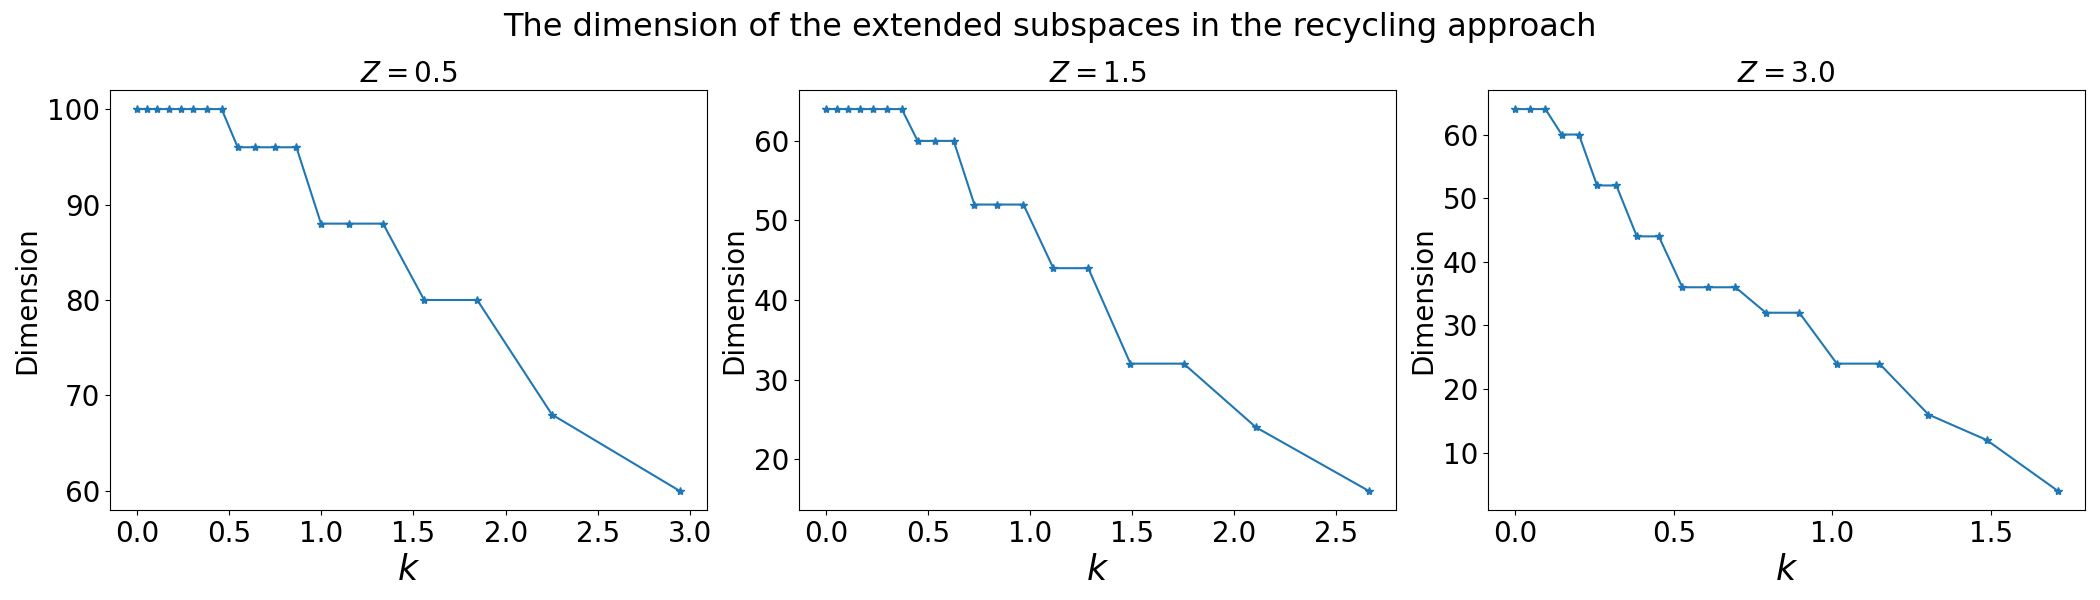
\includegraphics[width = \textwidth]{figures/Dimension_of_the_extended_subspace.png}
    \caption{The dimension of the extended subspace in the recycled approach for each wavenumber case, which is equal to the number of the recycled 
    eigenvectors plus the number of the residuals $\{\mathbf{r}_{i}\}_{i}$. The recycled eigenvector has the corresponding eigenvalue whose logarithm
    is larger than $10^{-5}$.  The scatterers are two spheres with equal radii $R = 1$ with distance $Z = 0.5$, 1.5 and 3.0.}
    \label{Dimension_of_the_extended_subspace}
\end{figure}

Table \ref{Table lists the logdet} lists the relative error for approximating the value of $\log\det(\mathsf{V}(\mathrm{i}k)\tilde{\mathsf{V}}(\mathrm{i}k)^{-1})$ 
computed via the inverse-free Krylov subspace method and standard Arnoldi method with or without recycling the subspace. {\color{teal}The reference value is computed by the 
direct dense computation of the log determinant.} It indicates that with the settings above, one 
can have at lease three significant digits accuracy.
 
\begin{table}[H]
    \centering
    \begin{tabular}{ |M{1.5cm}|M{2.0cm}|M{2.2cm} |M{2.2cm}|M{3cm}|M{3cm}|M{2.2cm}| } 
    \hline
    Distance $Z$ & Wavenumber $k$ &  Inverse-free (no recycling) & Inverse-free (recycling) & Standard Arnoldi (no recycling) & Standard Arnoldi (recycling)\\
    \hline
    \multirow{5}{4em}{$Z = 0.5$}   & 0        & $9.79\times 10^{-4}$  & $9.79\times 10^{-4}$  &$9.29\times 10^{-4}$ &$9.29\times 10^{-4}$\\ 
                                   & 0.0540   & $9.67\times 10^{-4}$  & $9.78\times 10^{-5}$  &$4.91\times 10^{-5}$ &$1.37\times 10^{-6}$\\ 
                                   & 0.111    & $1.22\times 10^{-3}$  & $2.79\times 10^{-5}$  &$5.29\times 10^{-5}$ &$5.17\times 10^{-6}$\\ 
                                   & 0.171    & $1.15\times 10^{-3}$  & $2.42\times 10^{-5}$  &$2.78\times 10^{-5}$ &$8.45\times 10^{-5}$\\ 
                                   & 0.236    & $1.25\times 10^{-3}$  & $9.10\times 10^{-6}$  &$1.12\times 10^{-4}$ &$2.76\times 10^{-5}$\\ 
    \hline
    \hline
    \multirow{5}{4em}{$Z = 1.5$}   & 0        & $9.48\times 10^{-4}$  & $9.54\times 10^{-4}$  &$3.41\times 10^{-7}$ &$3.41\times 10^{-7}$\\ 
                                   & 0.0540   & $1.02\times 10^{-3}$  & $2.87\times 10^{-4}$  &$5.89\times 10^{-7}$ &$3.97\times 10^{-8}$\\ 
                                   & 0.111    & $1.16\times 10^{-3}$  & $1.80\times 10^{-4}$  &$1.45\times 10^{-8}$ &$2.35\times 10^{-4}$\\ 
                                   & 0.171    & $1.25\times 10^{-3}$  & $1.35\times 10^{-4}$  &$2.70\times 10^{-6}$ &$1.06\times 10^{-4}$\\ 
                                   & 0.236    & $1.33\times 10^{-3}$  & $4.77\times 10^{-5}$  &$3.14\times 10^{-7}$ &$4.87\times 10^{-5}$\\ 
    \hline
    \hline
    \multirow{5}{4em}{$Z = 3.0$}   & 0        & $1.38\times 10^{-3}$  & $1.38\times 10^{-3}$  &$8.55\times 10^{-12}$ &$8.55\times 10^{-12}$\\ 
                                   & 0.0540   & $1.54\times 10^{-3}$  & $4.34\times 10^{-4}$  &$3.46\times 10^{-9}$  &$2.61\times 10^{-5}$\\ 
                                   & 0.111    & $1.81\times 10^{-3}$  & $2.89\times 10^{-4}$  &$5.02\times 10^{-10}$ &$5.43\times 10^{-7}$\\ 
                                   & 0.171    & $2.13\times 10^{-3}$  & $2.35\times 10^{-4}$  &$4.82\times 10^{-8}$  &$2.50\times 10^{-5}$\\ 
                                   & 0.236    & $2.54\times 10^{-3}$  & $2.13\times 10^{-4}$  &$5.07\times 10^{-9}$  &$1.59\times 10^{-5}$\\ 
    \hline
    \end{tabular}
    \caption{Relative error for approximating the value of $\log\det(\mathsf{V}(\mathrm{i}k)\tilde{\mathsf{V}}(\mathrm{i}k)^{-1})$ on the first five consecutive 
    quadrature points via the inverse-free Krylov subspace and standard Arnoldi methods with/without subspace recycled. The scatterers are two spheres with 
    equal radii $R = 1$ with distance $Z = 0.5$, 1.5 and 3.0. The sphere meshes are refined with size $h = 0.1$.}
    \label{Table lists the logdet}
    \end{table}
    
For large problems the dominating cost is that of the involved matrix-vector products with the integral operators. 
{\color{teal} In Figures \ref{matvec100} and \ref{matvec200} we plot the number of actual matvecs with the discretised matrix form $\mathrm{V}(\mathrm{i}k)$ for each individual algorithm.} The integral here has been discretized with {\color {teal} 20} quadrature
points. {\color{red} What is the number of quad points? You need to give this information.} {\color{red} Do you count the matvec with each component of the
2x2 block matrices $V_{ik}$ and $\tilde{V}_{ik}$ separately? Not clear from your description.} 

It shows that the recycling strategy significantly reduces the overall number of matrix-vector products necessary.

%To further compare the efficiency of these methods, we explore the number of matrix-vector multiplications for these methods on computing the Casimir energy
%and they are list inside Table \ref{4methods FLOP}. In addition, Figure \ref{matvec100} and Figure \ref{matvec200} plot the number of matrix-vector multiplications
%that we need to compute the Casimir energy between two spheres with distance $Z = 0.5$, 1.5 and 3.0 by using these methods with or without recycling the subspaces.
%One can notice that the methods with recycling the subspace  have similar number of matvec and they also have smaller number of matvec than the non-recycling methods.
%Therefore, for all the numerical experiments in Section \ref{Numerical experiments}, we would apply the methods with subspaced recycled to compute the Casimir energy.
%\begin{table}[H]
%    \centering
%\begin{tabular}{ |P{4cm}|P{4cm}|P{4cm}|P{4cm}|  }
%    \hline
%    \multicolumn{2}{|c|}{Inverse-free Krylov subspace method}& \multicolumn{2}{c|}{Standard Arnoldi method} \\
%    \hline
%   Without recycling &  With recycling & Without recycling& With recycling\\
%    \hline
%    $(2m - 1)N$  & $(2m - 1) + 2\sum_{i = 1}^{N-1}s_{i}$   & $(m - 1)N$ &   $(m - 1) + 2\sum_{i = 1}^{N-1}s_{i}$ \\
%    \hline
%   \end{tabular}
%   \caption{The number of matrix-vector multiplications inside the inverse-free Krylov subspace and standard Arnoldi methods with or without recycling subspaces.
%   $N$ is the number of wavenumbers, $m$ is the dimension of the Krylov subspace for the first wavenumber (in recycling case); for all the wavenumbers (in non-recycling case),
%   and $s_{i}$ is the number of the extracted eigenvectors 
%   for the $i$th wavenumber's case (in recycling case).}
%   \label{4methods FLOP}
%\end{table}
\begin{figure}[H]
    \centering
    \hspace*{-1.5cm}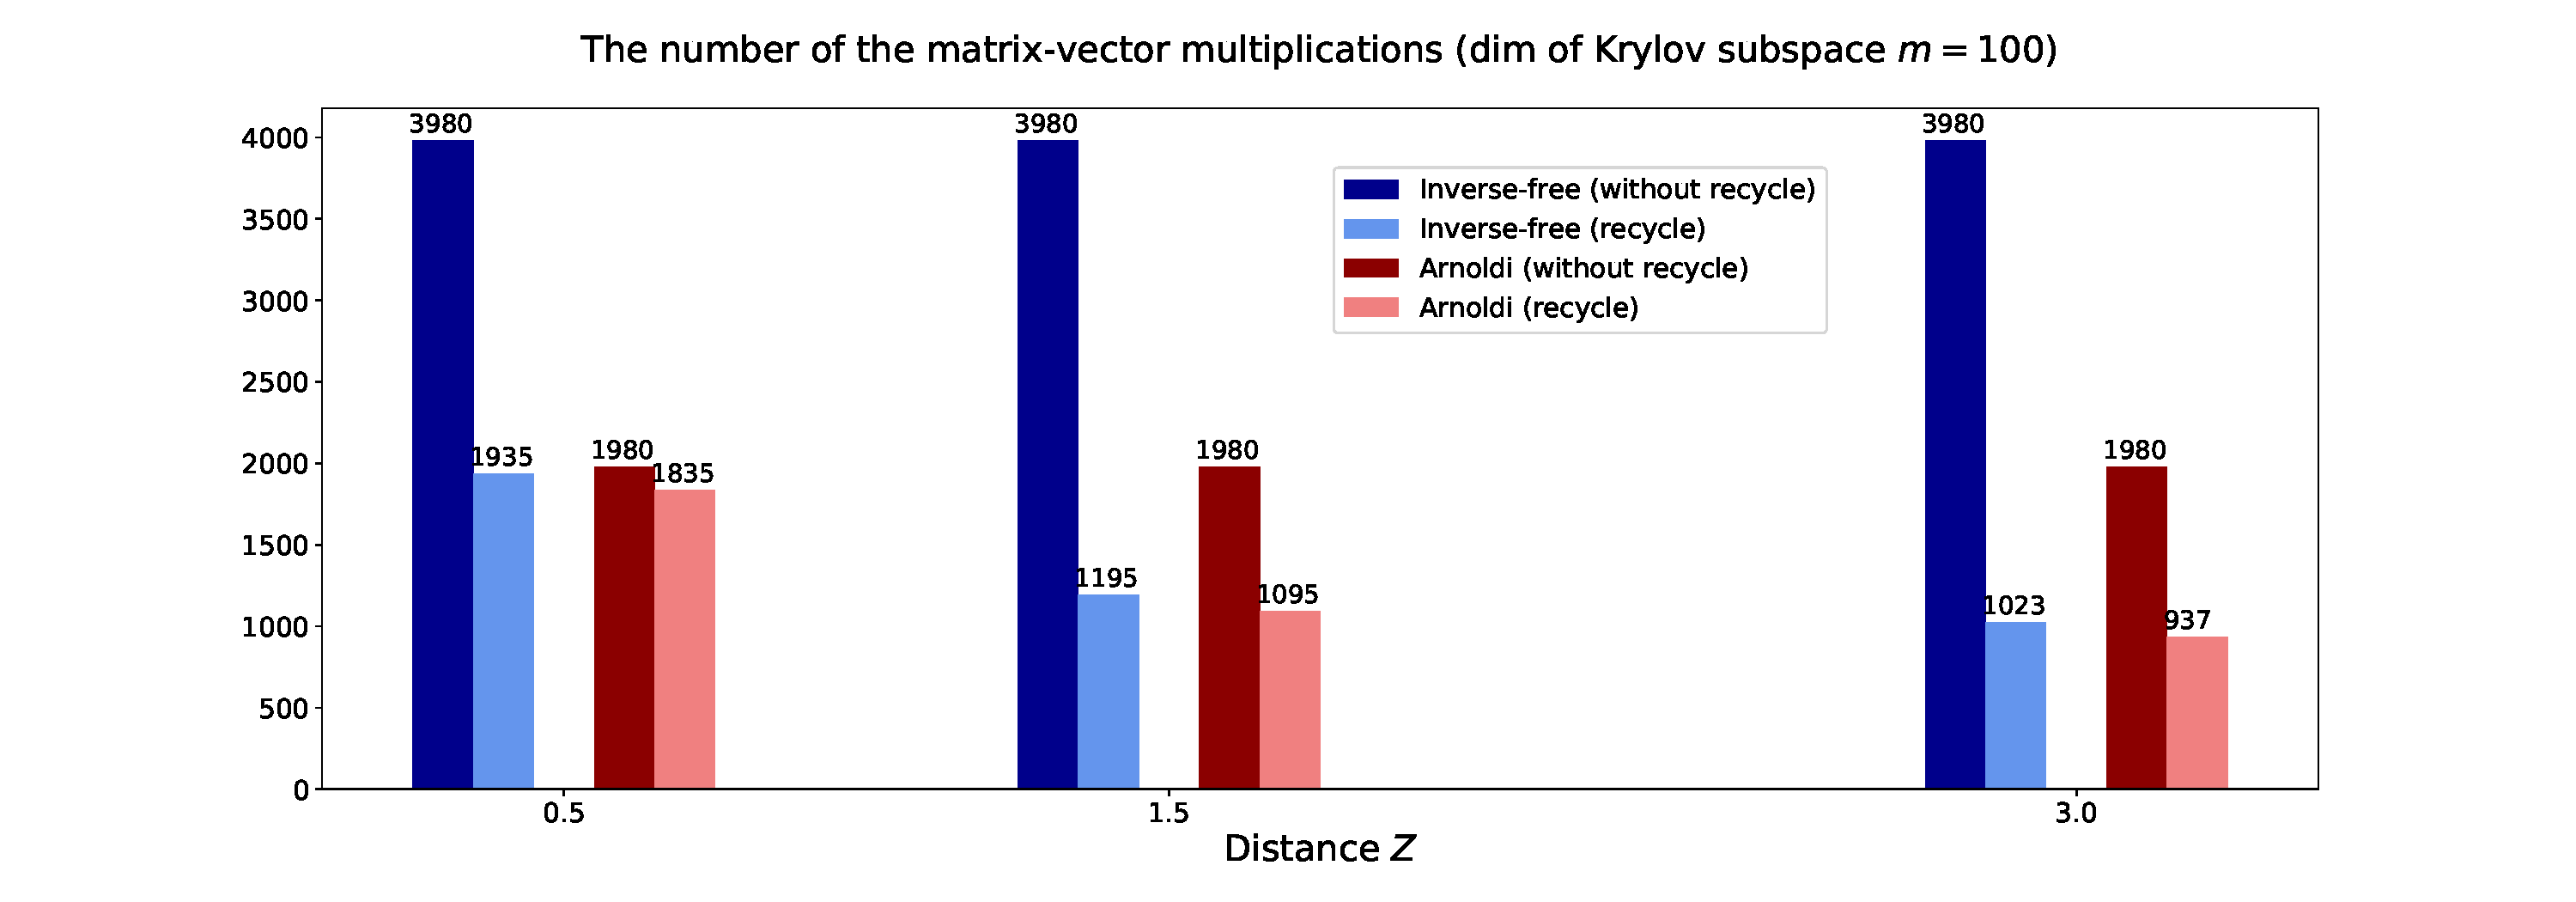
\includegraphics[scale = 0.4]{figures/matvec_100.pdf}
    \caption{The number of the matrix-vector products inside inverse-free and standard Arnoldi methods with or without recycling subspace. The scatterers are two spheres with equal radii $R = 1$ and distance $Z$ is 0.5, 1.5 and 3.0. The dimension of the Krylov subspace is set as $m = 100$.}
    \label{matvec100}
\end{figure}

\begin{figure}[H]
    \centering
    \hspace*{-1.5cm}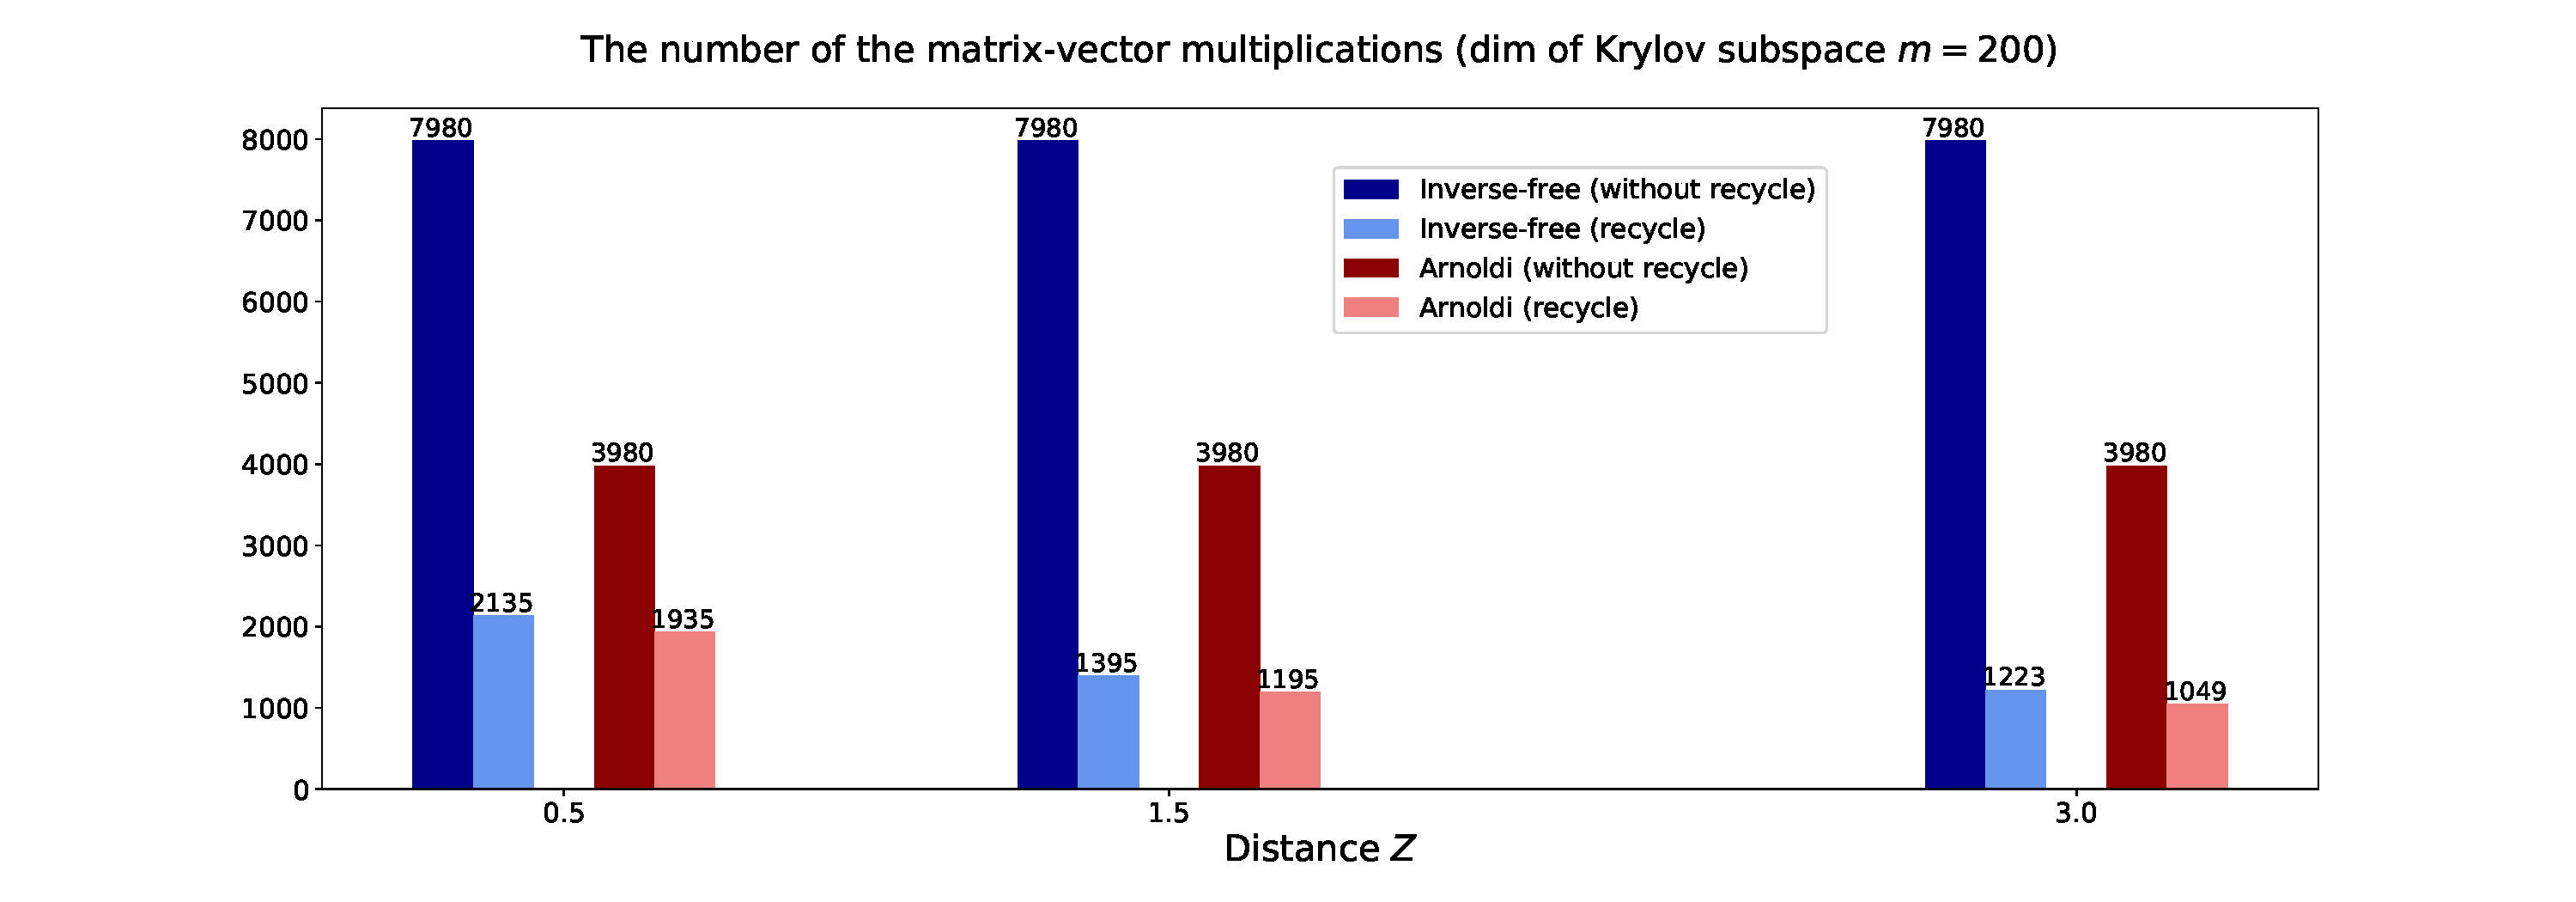
\includegraphics[scale = 0.4]{figures/matvec_200.pdf}
    \caption{The number of the matrix-vector products inside inverse-free and standard Arnoldi methods with or without recycling subspace. The scatterers are two spheres with equal radii $R = 1$ and distance $Z$ is 0.5, 1.5 and 3.0. The dimension of the Krylov subspace is set as $m = 200$.}
    \label{matvec200}
\end{figure}

%Note that for the recycled methods Algorithm \ref{Alg for computing the evals kry recycled}-\ref{Alg for computing the evals arno recycled}
%we apply different rules for extracting the eigenvectors. For  
%is different which depends on the 

%For the standard Arnoldi method,  it can be noticed that the number of FLOP is cubicly increasing with the size of the matrix 
%no matter the subspace is recycled or not. For the inverse-free Krylov subspace methods, as the wavenumber $k$ increases, the number of the extreme eigenvalues
%decreases which makes the number of extracted eigenvectors decreases as well. Therefore, for the large-scale problems, the inverse-free Krylov subspace method with 
%subspaces recycled would be applied to compute the Casimir energy with lower complexity and desired accuracy.
